\section{Case Study: Verification of \texttt{[T]::binary\_search}}
\label{sec:binary_search}

As a first test of the translation tool, we set out to verify the correctness
the binary search implementation in the Rust standard library, an algorithm of
medium complexity.

Before we can even the algorithmic complexity, we have to cope with the
design complexity of a real-world library. The public implementation of the
method on any slice type can be found in the \rust{collections} crate.

\begin{minted}{rust}
use core::slice as core_slice;

impl<T> [T] {
  ...

  /// Binary search a sorted slice for a given element.
  ///
  /// If the value is found then `Ok` is returned, containing the
  /// index of the matching element; if the value is not found then
  /// `Err` is returned, containing the index where a matching
  /// element could be inserted while maintaining sorted order.
  ///
  /// ...
  pub fn binary_search(&self, x: &T) -> Result<usize, usize>
    where T: Ord {
    core_slice::SliceExt::binary_search(self, x)
  }
}
\end{minted}

As can be seen from the method's documentation and signature, it
is very general: The method works on all slices whose element type implements the
\rust{Ord} trait, and it returns information in both the success and the failure
case. The implementation, however, turns out to be merely a redirection to a
trait method in the base crate \rust{core}. The trait is only implemented
on the slice type.

\begin{minted}{rust}
pub trait SliceExt {
  type Item;

  fn binary_search(&self, x: &Self::Item) -> Result<usize, usize>
    where Self::Item: Ord;
  fn len(&self) -> usize;
  fn is_empty(&self) -> bool { self.len() == 0 }
  ...
}

impl<T> SliceExt for [T] {
  type Item = T;

  fn binary_search(&self, x: &T) -> Result<usize, usize> where T: Ord {
    self.binary_search_by(|p| p.cmp(x))
  }
  ...

}
\end{minted}

This indirection seems pointless at first, but follows from a technical
restriction: There may be at most one \rust{impl} block for a primitive type
like \rust{[T]}. Because the \rust{core} crate does not depend on the existence
of a heap allocator, but some methods on \rust{[T]} like its merge sort
implementation do need dynamic allocation, the \rust{impl} block is only
declared in the later \rust{collections} crate. Since \rust{binary_search} does
not need an allocator, it should still reside in \rust{core}, and instead is
associated to the slice type via the helper trait.

\begin{listing}[!bt]
\begin{minted}{rust}
fn binary_search_by<'a, F>(&'a self, mut f: F) -> Result<usize, usize>
    where F: FnMut(&'a T) -> Ordering
{
    let mut base = 0usize;
    let mut s = self;

    loop {
        let (head, tail) = s.split_at(s.len() >> 1);
        if tail.is_empty() {
            return Err(base)
        }
        match f(&tail[0]) {
            Less => {
                base += head.len() + 1;
                s = &tail[1..];
            }
            Greater => s = head,
            Equal => return Ok(base + head.len()),
        }
    }
}
\end{minted}
  
\caption{Implementation of the \rust{binary_search_by} method. A subslice
  \rust{s} of \rust{self} is iteratively bisected until it is empty or the
  element has been found. The \rust{tail[1..]} \emph{slicing syntax} is
  syntax sugar for \rust{tail.index(RangeFrom{start: 1})}.}
\label{lst:binary_search_by}
\end{listing}

This final version of \rust{binary_search}, which we represent as
\rust{core::<[T] as SliceExt>::binary_search}, is implemented by way of a more
general method \rust{binary_search_by} that takes a comparison function instead
of being constrained to \rust{Ord} (\autoref{lst:binary_search_by}). This
method, finally, turns out to be more abstract than one might expect: instead of
the standard implementation that iteratively reduces the search range via two
indices, the range is represented as a subslice and manipulated via high-level
slice methods such as \rust{split_at}. The reasoning behind this is a great show
case for Rust's zero-cost (or even negative-cost, in this case) abstractions
philosophy -- the abstract implementation actually surpasses the direct
implementation in terms of efficiency because it helps the compiler to eliminate
all bounds checks in it. It also elegantly avoids the common
pitfall\footnote{https://research.googleblog.com/2006/06/extra-extra-read-all-about-it-nearly.html}
of a potential integer overflow in less abstract code like \rust{mid = (low + high) / 2}.

\begin{sidewaysfigure}
  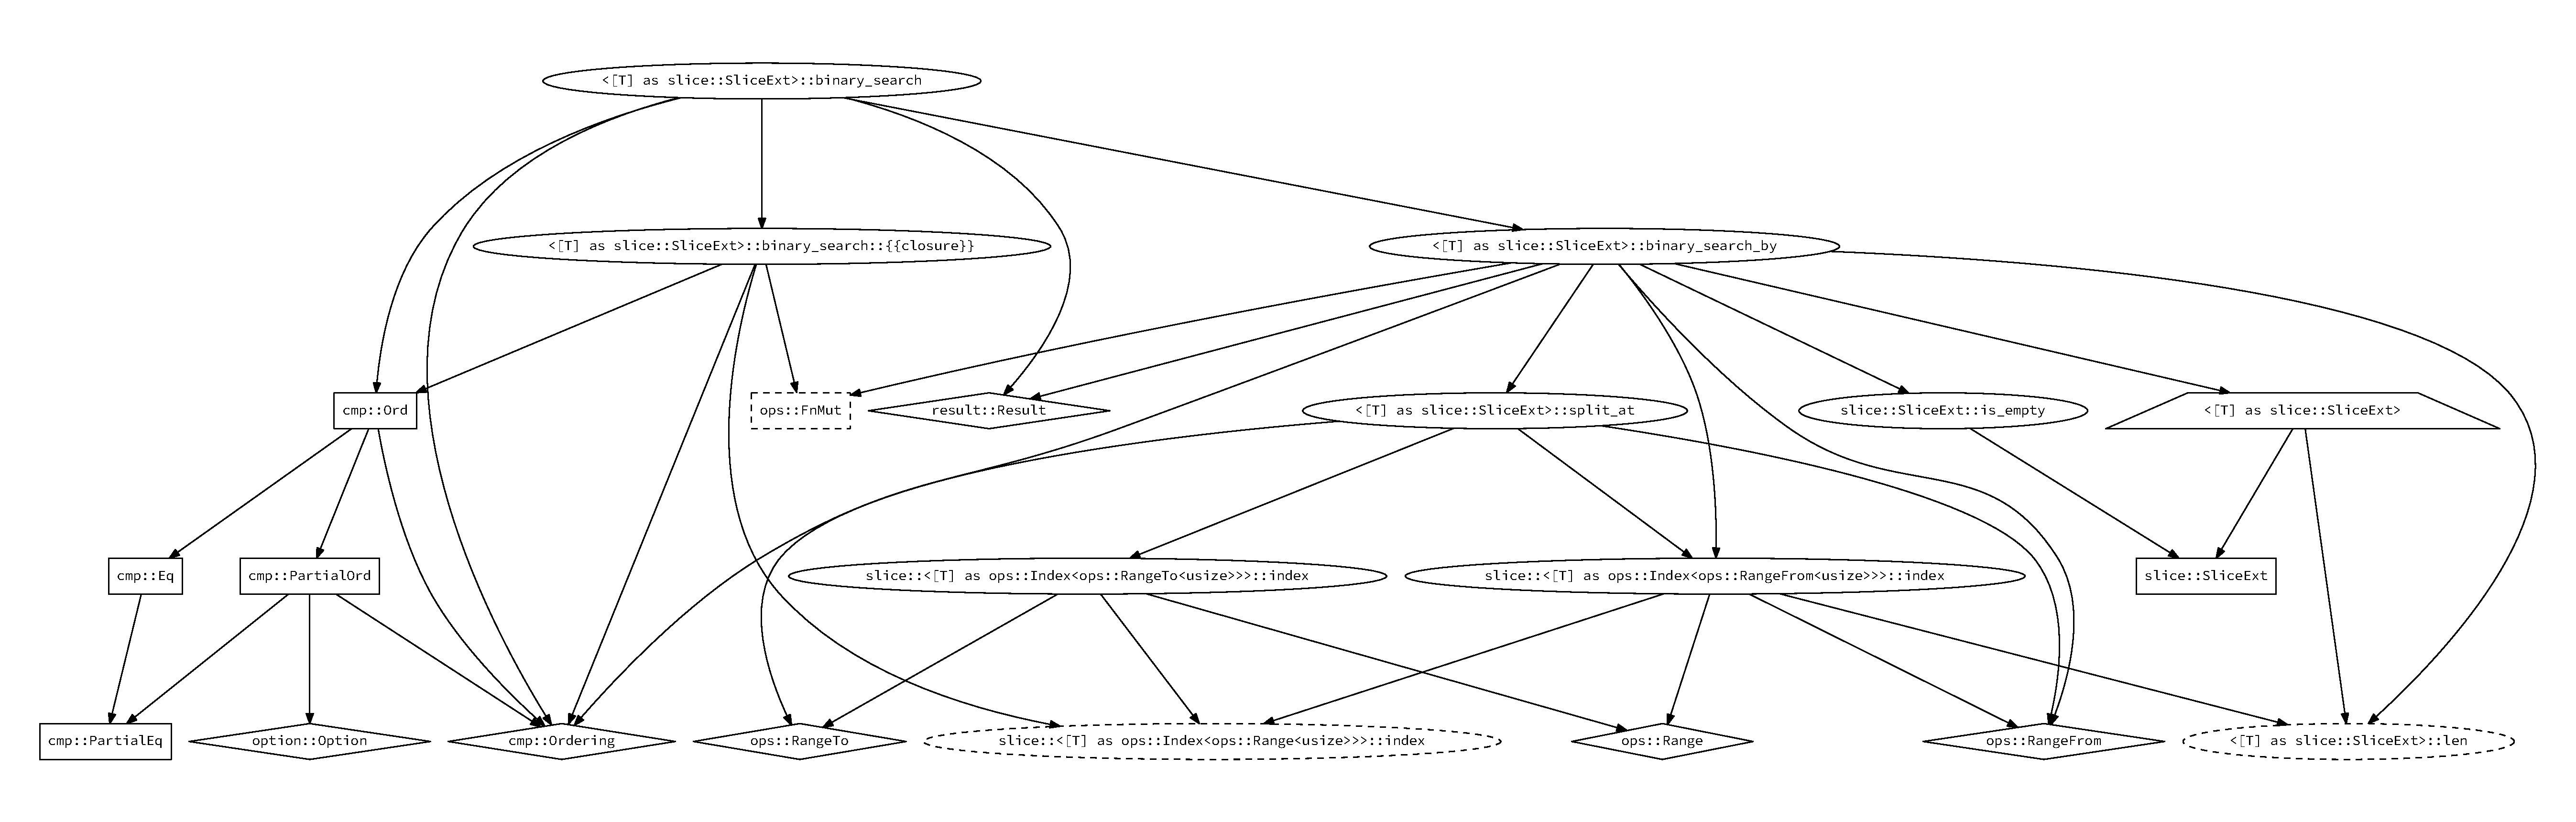
\includegraphics[width=\textheight]{deps}
  \caption[A complete graph of the dependencies of \rust{binary_search}]{A
    complete graph of the translation dependencies of \rust{binary_search} in
    the \rust{core} crate,
    distinguishing between \tikz[baseline=-0.3em]\node[draw, shape=ellipse] {functions};,
    \tikz[baseline=-0.3em]\node[draw, shape=rectangle] {types};,
    \tikz[baseline=-0.3em]\node[draw, shape=diamond, aspect=2] {traits};,
    and \tikz[baseline=-0.3em]\node[draw, shape=trapezium] {trait
      implementations};. Axiomatized items that use unsafe code in the original
    implementation are marked by dashed borders. Because
    we eagerly resolve trait method calls where possible, such as to the
    \rust{index} method of \rust{Index<RangeFrom<usize>>} for \rust{[T]}, we can
    avoid some dependencies like the full \rust{Index} implementation for
    \rust{[T]}, and even the trait itself.
  }
  \label{fig:deps}
\end{sidewaysfigure}

For our purposes, the abstract implementation primarily means a fair number of
additional dependencies we have to support and inspect~(\autoref{fig:deps}). All
in all, \rust{binary_search} turned out to be an ideal first test not only because
of its algorithmic complexity, but also because of its use of numerous Rust
language features including enums, structs, traits with associated types and
default methods, higher-order functions, and loops.

When trying to translate the \rust{binary_search} method including its
dependencies, we will not get back a working definition at first. Our tool
refuses to translate some dependencies because they use unsafe code, as marked
in \autoref{fig:deps}. We will have to translate these functions manually,
basically adding the correctness of their translation as axioms to the project.

Apart from our custom translation of \rust{FnMut} we discussed in
\autoref{sec:lambda}, both axiomatized functions operate on slices and are straightforward to
implement using our identification of slices with Lean lists.

\begin{minted}{lean}
definition «[T] as core.slice.SliceExt».len {T : Type₁} (self : slice T) : sem nat :=
return (list.length self)

definition core.«[T] as core.ops.Index<core.ops.Range<usize>>».index {T : Type₁} (self : slice T) (index : Range usize) : sem (slice T) :=
if Range.start index ≤ Range.«end» index ∧ Range.«end» index ≤ list.length self
then return (list.firstn (Range.«end» index - Range.start index) (list.dropn (Range.start index) self))
else mzero
\end{minted}

